\section{TRANSIENT THERMAL ANALYSIS}
\normalsize{Transient thermal analysis is carried out to assess the different time duration at which:
\begin{itemize}
    \item the maximum operational temperature of the parts is exceeded.
    \item the thermal equilibrium is atteigned.
    \item the effect of high temperature gradient on the evolution of the part temperature.
\end{itemize}
Those points will help us better understand the thermal bahevior of the tile and maybe allow to set time constraints on pulse duration to avoid damaging the assembly.}
\subsection{Analysis for HE1 to HE4 pulse duration}
\normalsize{During the operational life \acrshort{W7-X}, the device will be used in different operational phases. Each operational phase has different and specific operational parameters such as the plasma pulse duration \cite{Lorenz2020}. The plasma pulse duration are called $HE$ and have a number to caracterize them. There are 5 different pulse length (noted $HE1$ to $HE4$).}
\\
\begin{figure}[h!]
    \label{fig_5_12} 
    \centering
    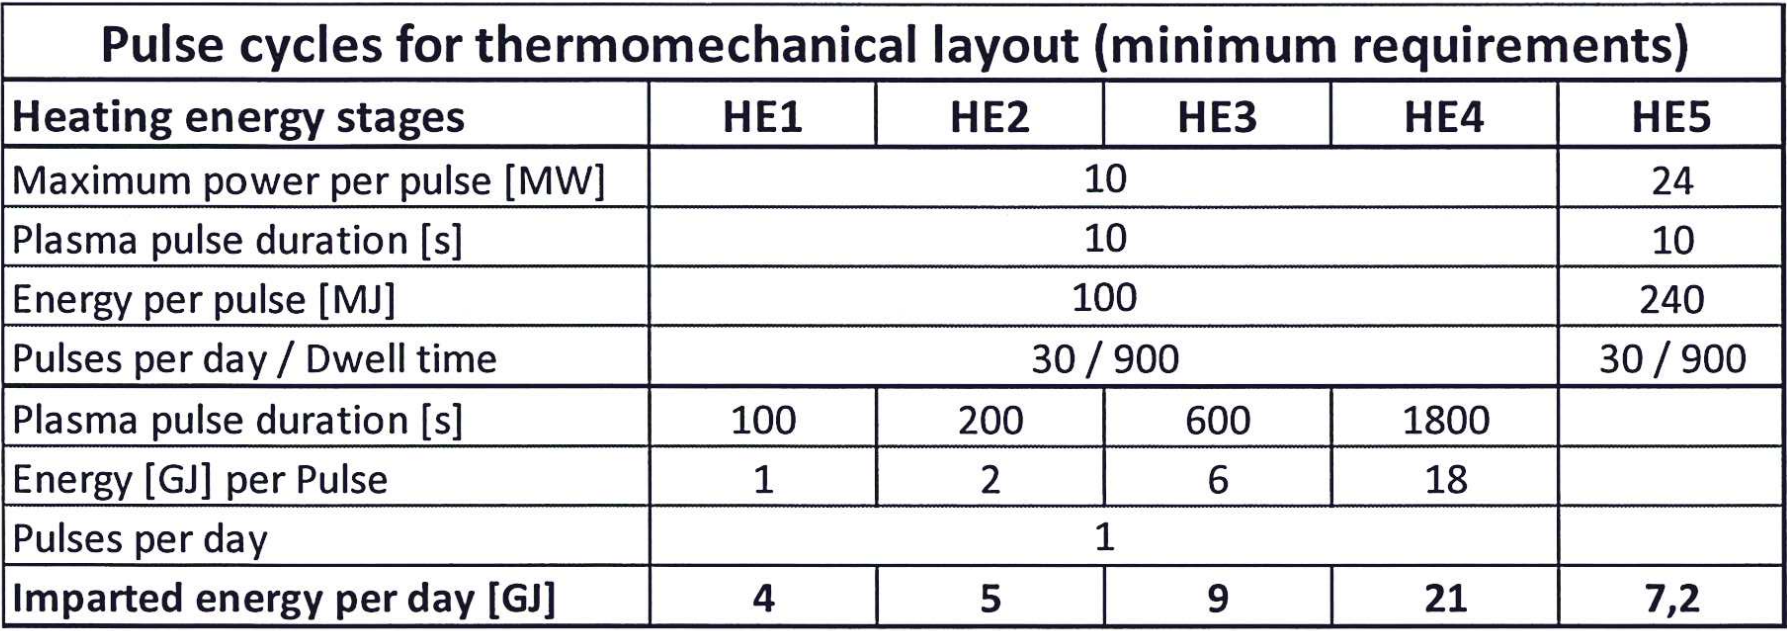
\includegraphics[width=1\textwidth]{figures/pulselengthtable.png}
    \caption{\it Table of the pulse durations \cite{Lorenz2020}}
\end{figure}
\\
\normalsize{\indent For \acrshort{OP2}, the next operation phase of \acrshort{W7-X}, the nest pulse duration is {\bfseries $HE2$} (in an ideal case, the parts of the tile assembly should not exceed their maximum temperature). The tile assembly will simulated for all cases except $HE5$. The pulse is modelled by a step function and the boundary conditions are the same as the one for the static thermal analysis \ref{Load case influence on thermal behavior}.}
\\
\break
\normalsize{\indent It is also important to calculate a minimum timestep to avoid calculation errors. For this, it is necessary to set a Fourier number and use its definition to calculate the minimum timestep. We set the Fourier number $Fo$ to be 10 (enough time has passed to the tile to reach equilibirum temperature). It is important to note that this number is a placeholder and is assumed to be that value.}
\\
\break
\normalsize{\indent The solver is set for 5 loadcases:
\begin{itemize}
    \item AAAA
\end{itemize}
}
\subsection{Analysis for HE1 pulse length and cooldown}